\subsubsection{Mouse visual cortex spike data during visual stimulation}
\label{subsubsection:rebuttal_allen_stimulus_features}

To test whether NLDisco latents also represent environmental variables, we analyze visual stimulus features in the Allen Institute Visual Coding Neuropixels session 732592105~\citep{siegle_2021_allen_datasets}, the recording used for \autoref{figure:model_eval}. As in the other experiments, the model never sees stimulus labels; they are used only to define the data split and to interpret and score latents.

\paragraph{Dataset.}
The recording contains 201 units in five visual cortical areas (VISp 64, VISal 44, VISpm 37, VISrl 37, VISl 19; area of each unit's peak channel), binned into 182,868 50-ms bins. The session presents Gabor patches at 81 positions on a $9\times9$ grid (10$^\circ$ spacing), full-field flashes, drifting gratings (8 directions, 5 temporal frequencies), static gratings (6 orientations, 5 spatial frequencies, 4 phases), 118 natural images, two natural movies, and spontaneous activity. We label each bin with the stimulus shown 50 ms before its midpoint, a fixed delay between stimulus and neural response used for all features. Among delays of 0, 50, 100, and 150 ms, 50 ms gives the highest (or, for the movie feature, equal-highest) training-split \metric{AUROC} for each selected latent. We exclude 5,933 bins that overlap the session's annotated invalid intervals.

\paragraph{Held-out split.}
We split stimulus presentations rather than bins. Each Gabor, flash, grating, or image presentation, together with any gray interval that follows it, forms one split unit, as does each natural-movie repeat and each 10-s piece of spontaneous activity. Within each stimulus type, a random 20\% of the 16,537 units is held out (seed 0), leaving 142,108 training bins and 34,394 held-out bins. Model fitting, normalization statistics, threshold calibration, latent inspection, delay choice, and feature definitions use the training split only; all scores and tuning plots in \autoref{figure:rebuttal_allen_features} and \autoref{table:rebuttal_allen_metrics} use the held-out split unless marked otherwise.

\paragraph{Model.}
The SED follows \autoref{figure:model_eval}: single 50-ms bins ($S=1$) with a linear encoder, $L=3$ Matryoshka levels $(D_\ell,k_\ell)\in\{(128,12),(224,24),(320,36)\}$, and $B=1024$, trained for 30 epochs (4,170 Adam updates) with the learning-rate schedule described above. As in the Aeon analysis, unit counts are standardized with training-split statistics and reconstructed with MSE and an identity output activation. This model reconstructs held-out activity with variance-weighted \metric{R^2} $0.939$, with mean \metric{L0} $36.4$ and no dead latents. We also trained the same model on unstandardized counts (51 dead latents and 12 latents active in more than half of training bins) and a 200-ms window variant ($S=4$, held-out \metric{R^2} $0.603$); we use the standardized single-bin model because its latents show the clearest stimulus tuning.

\paragraph{Feature discovery.}
For each of the 320 latents, we compute activation probabilities and the association metrics on training bins for 473 candidate conditions within each stimulus type: every value of each stimulus parameter (for gratings, also every pair of the first two parameters), every Gabor position, every natural image, and every 1-s segment of each natural movie. We then inspect tuning maps of the highest-scoring latents and fix four feature descriptions, one per stimulus type with the clearest tuning:
\begin{enumerate}[leftmargin=*,itemsep=2pt]
    \item \textit{Gabor at (10$^\circ$, 10$^\circ$)}: a Gabor patch (20$^\circ$ diameter) centered at azimuth 10$^\circ$ and elevation 10$^\circ$, compared with Gabors at the other 80 positions (latent 196).
    \item \textit{Drifting grating at $\geq$8 Hz}: a full-field grating drifting at 8 or 15 Hz in any direction, compared with 1--4 Hz gratings, blank sweeps, and the gray intervals between gratings (latent 65).
    \item \textit{Natural image 19}: image 19 of the 118 natural images, compared with the other images and blank sweeps (latent 70).
    \item \textit{Natural movie 3, second 115}: frames 3,450--3,479 of the 120-s natural movie 3, compared with the rest of the movie (latent 112).
\end{enumerate}
Latent indices are zero-based in the $D=320$ dictionary. A latent is active when $z>0$, and \metric{AUROC} uses its continuous activation values (\hyperref[subsubsection:latents_evaluation_details]{\ref*{subsubsection:latents_evaluation_details}}).

\paragraph{Results.}
All four features generalize to held-out presentations (\autoref{table:rebuttal_allen_metrics}), with held-out \metric{AUROC} between $0.770$ and $0.972$ and \metric{Sel} between $0.769$ and $0.920$. The Gabor latents form spatially localized receptive-field maps, and further latents tile other parts of the visual field (\autoref{figure:rebuttal_allen_features}a); scored at their training peaks, latents 84, 49, and 22 reach held-out \metric{AUROC} $0.819$, $0.917$, and $0.816$. Latent 65 increases its activation probability with grating temporal frequency across directions and is nearly silent during gray screens (\autoref{figure:rebuttal_allen_features}b). Latent 70 is active for 80\% of held-out image-19 bins but for 7\% of other natural-scene bins (\autoref{figure:rebuttal_allen_features}c), and latent 112 reproduces its training-split time course through natural movie 3 on the held-out repeat (\autoref{figure:rebuttal_allen_features}d). The held-out movie scores use one repeat of natural movie 3 (20 bins in the condition). Together, these latents show that NLDisco, trained without stimulus labels, learns individual latents that represent stimulus position, temporal frequency, and specific natural images and movie segments.

\begin{figure}[!htbp]
    \centering
    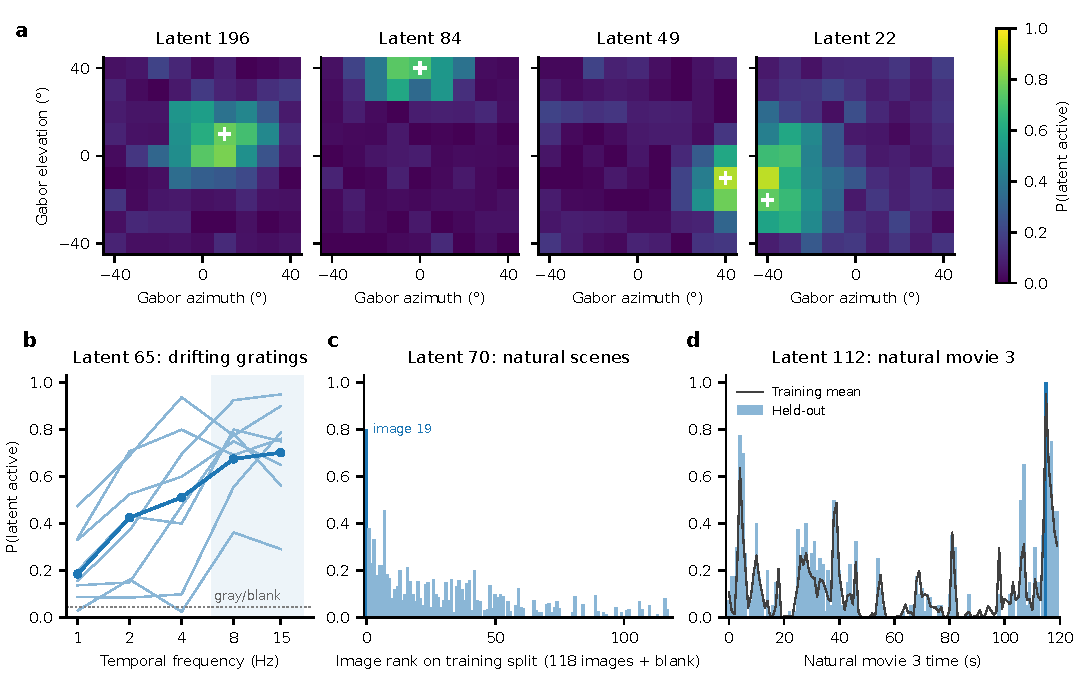
\includegraphics[width=\linewidth]{figures/rebuttal/change04_allen/allen_stimulus_features.pdf}
    \caption{\textbf{Visual stimulus features in mouse visual cortex.} Held-out activation probabilities of NLDisco latents ($D=320$, $k=36$) in Allen session 732592105, with each 50-ms bin labelled by the stimulus shown 50 ms earlier. (\textbf{a}) Receptive-field maps over the 81 Gabor positions for latent 196 (scored at 10$^\circ$, 10$^\circ$) and latents 84, 49, and 22; crosses mark each latent's peak position on the training split. (\textbf{b}) Latent 65 across drifting-grating temporal frequencies for each of the 8 directions (thin lines) and pooled over directions (thick line); shading marks the scored condition and the dotted line the activation probability during blank sweeps and gray intervals. (\textbf{c}) Latent 70 across the 118 natural images and blank, ordered by training-split activation probability; the dark bar is image 19. (\textbf{d}) Latent 112 across 1-s segments of natural movie 3 on the held-out repeat (bars) and averaged over training repeats (line); the dark bar is second 115.}
    \label{figure:rebuttal_allen_features}
\end{figure}

\begin{table}[!htbp]
    \centering
    {\small\setlength{\tabcolsep}{3pt}\renewcommand{\arraystretch}{1.12}
    \begin{tabular*}{\linewidth}{@{\extracolsep{\fill}}llrrrrrr@{}}
\toprule
Split & Latent & \metric{Cov} & \metric{Spec} & \metric{Sel} & \metric{AUROC} & Bins in $C$ & Bins in $\neg C$ \\
\midrule
\multicolumn{8}{l}{\textit{Gabor at (10$^\circ$, 10$^\circ$)}} \\
Train (80\%) & 196 & 0.893 & 0.847 & 0.853 & 0.909 & 150 & 13,150 \\
Held-out (20\%) & 196 & 0.769 & 0.841 & 0.828 & 0.838 & 65 & 3,273 \\
\midrule
\multicolumn{8}{l}{\textit{Drifting grating at $\geq$8 Hz}} \\
Train (80\%) & 65 & 0.772 & 0.780 & 0.779 & 0.812 & 7,685 & 22,401 \\
Held-out (20\%) & 65 & 0.689 & 0.793 & 0.769 & 0.770 & 1,841 & 5,725 \\
\midrule
\multicolumn{8}{l}{\textit{Natural image 19}} \\
Train (80\%) & 70 & 0.865 & 0.933 & 0.928 & 0.917 & 170 & 22,313 \\
Held-out (20\%) & 70 & 0.800 & 0.930 & 0.920 & 0.882 & 60 & 5,598 \\
\midrule
\multicolumn{8}{l}{\textit{Natural movie 3, second 115}} \\
Train (80\%) & 112 & 0.950 & 0.891 & 0.897 & 0.946 & 160 & 18,663 \\
Held-out (20\%) & 112 & 1.000 & 0.864 & 0.880 & 0.972 & 20 & 3,847 \\
\bottomrule
\end{tabular*}
}
    \caption{\textbf{Association scores for the four visual stimulus features.} Each row group reports one NLDisco latent ($D=320$, $k=36$) on the training presentations used for discovery and on the held-out presentations. \metric{Cov}, \metric{Spec}, and \metric{Sel} use native positive activation; \metric{AUROC} uses continuous activation values. Bins are 50-ms bins labelled by the stimulus shown 50 ms earlier; neighboring bins within a presentation are not independent observations.}
    \label{table:rebuttal_allen_metrics}
\end{table}
